% chapters/intro.tex 
%	First chapter in VSRP Report.

Shape from Shading (SfS) is a 3D image reconstruction technique, in which the shape of a 3D object (output) is retrieved from a 2D image (input). The 2D image is a light intensity map of the 3D object, which is a grayscale image. The intensity map is obtained by flashing light over the object from a particular point (known \textit{apriori}) to illuminate the object. Then a mathematical model is constructed to relate the pixel intensity in the input image to obtain the depth information of the 3D surface. Figure (\ref{fig:1}) gives a flow chart of the process in SfS.

\begin{figure}[h!]
	\centering
	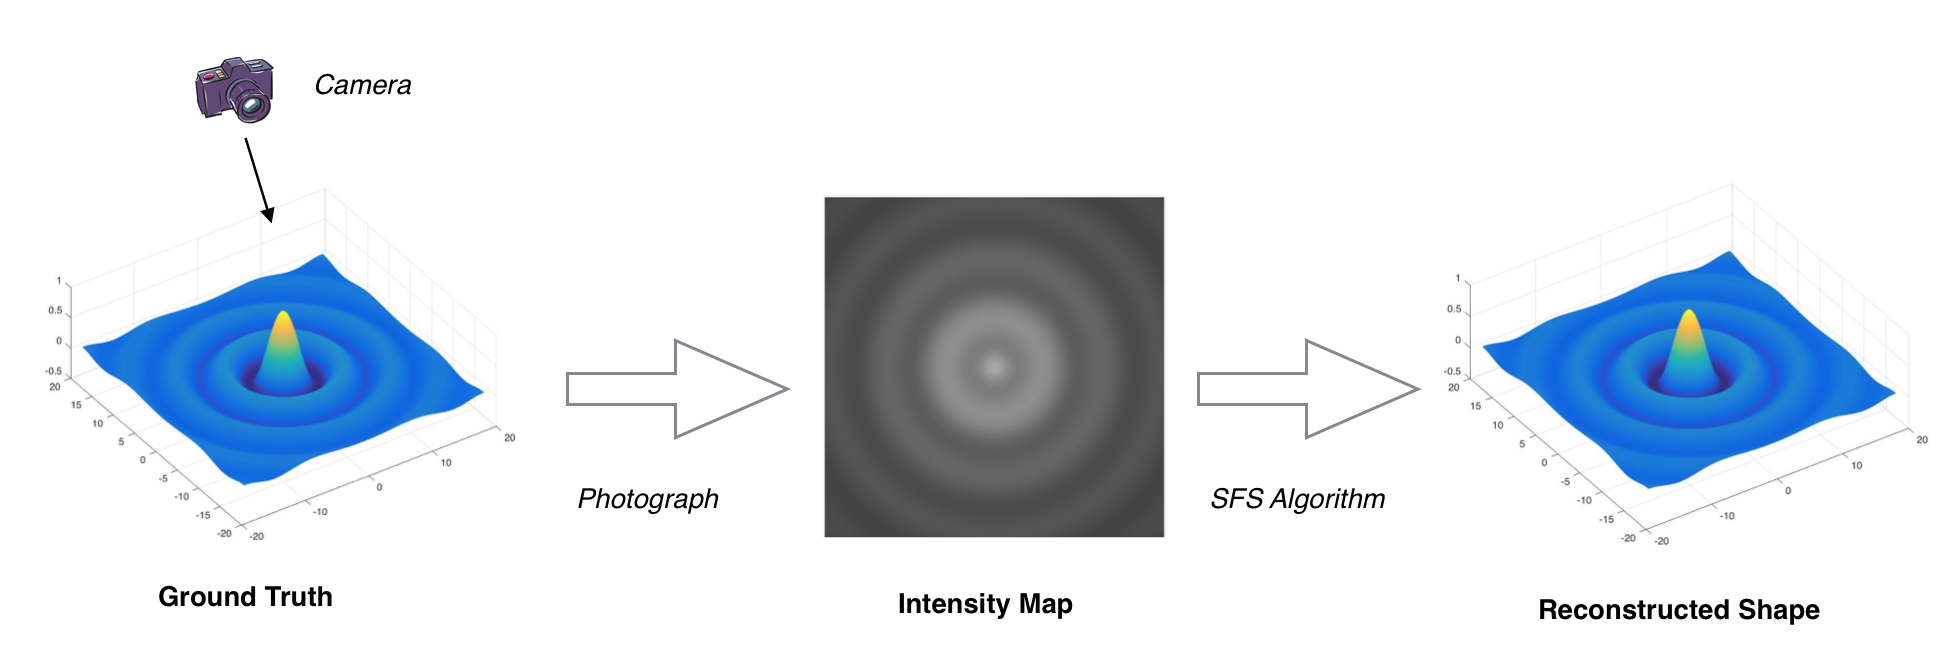
\includegraphics[width = 15.5cm]{images/flow.png}
	\caption{\textbf{Shape from Shading :} The \emph{ground truth} is the original object and SfS attempts to reconstruct it, just from knowing the \textit{Intensity map}}
	\label{fig:1}
\end{figure}

\noindent
The relation between the intensity of a pixel and the height of our reconstructed surface is given by a PDE. K.P.Horn\cite{horn} has given an eikonal equation type approach to formulate the Shape from Shading problem. This is known as the \textbf{orthographic projection model}. Rouy and Tourin\cite{rouy} came up with a viscosity solution approach to the model, and constructed an upwind type numerical scheme to solve the Eikonal type equation. Though this model was simple and effective, it suffered from a disadvantage because of singular points (More on singular points will be discussed in the coming chapters), where uniqueness of the solution is lost.\\

\noindent
 Prados and Faugeras\cite{prados2} came up with a much more realistic model that takes care of this difficulty. To solve the resulting PDE, Prados and Faugeras\cite{prados1} formulates a minimization approach, although solving the PDE using numerical techniques works as good. In this work, we present a numerical method to solve the PDE that arises due to Prados's work without using the minimization approach. Some applications of shape from shading can be found in \cite{prados1}\\
 
 \noindent
 This report is divided into 6 chapters. Chapter 2 introduces the reader to Hamilton Jacobi Equations (HJE), which is the backbone of Shape from Shading. This chapter discusses the need for viscosity solutions, and some existence, uniqueness results. Chapter 3 deals with the development of Orthographic Projection Model and discusses the notion of singular points and some ways to overcome the problem. Chapter 4 discusses the Perspective Projection approach to SfS problems and presents some existence and uniqueness results. Chapter 5 deals with the construction of some numerical schemes to solve the Eikonal Equation in a variety of domains, using the immersed boundary method. Numerical schemes to solve the SfS problems are discussed and the stability of these schemes are explained. Chapter 6 presents the results of some numerical experiments that were conducted on a variety of synthetic images to illustrate SfS.
